\begin{enumerate}
\def\labelenumi{\arabic{enumi}.}
\item
  I del 2 beregnes \(F_{res}\), der er konstant. Tegn \((a, F_{res})\)
  grafen. Bestem liniens hældning og sammenlign denne med den samlede
  masse\\
  Vi starter med at finde accelerationen for loddene i de forskellige
  måleserier. Dette gør vi ved at plotte hastighedsfunktionen og finde
  hældningskoefficienten. Da den er accelerationen\\
  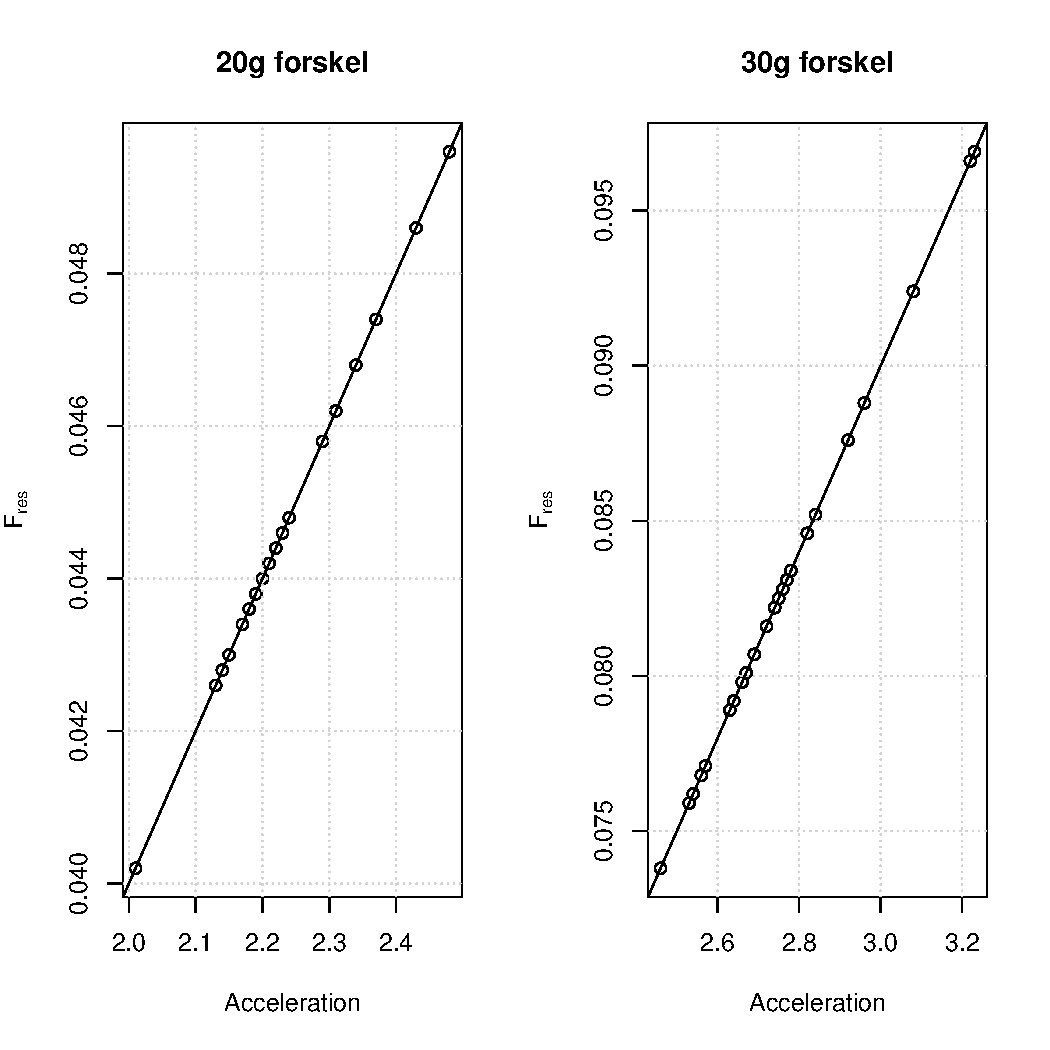
\includegraphics{opgave1.pdf} Vi har fundet accelerationerne til at
  være \(2.213\) og \(2.760\)\\
  Nu kan vi så finde \(F_{res}\) for de to punkter og plotte dem i et
  diagram.\\
  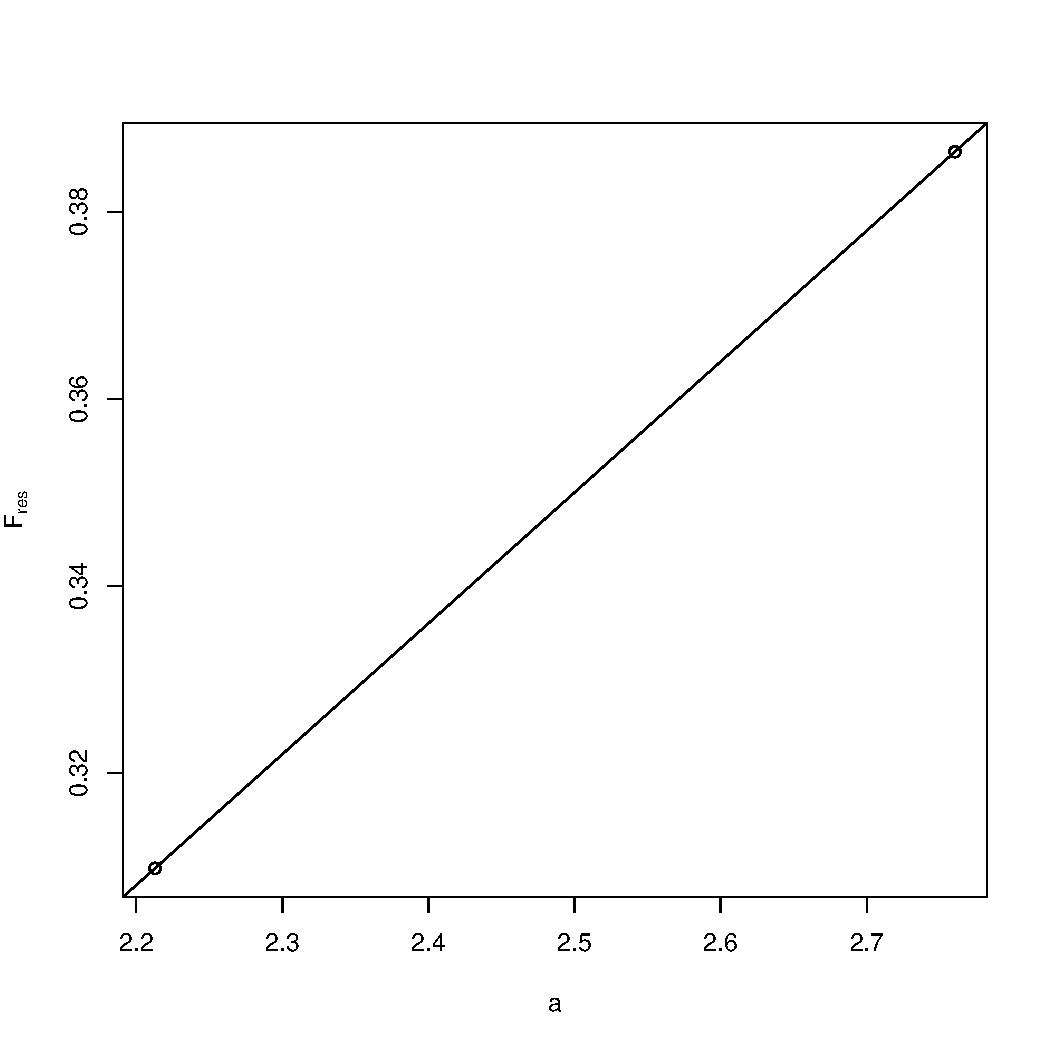
\includegraphics{opgave1acc.pdf} Vi har fundet hældningen til at være
  \(0.14\) og da \(F_{res}=(M_1+M_2) \cdot a\) svarer det til en samlet
  masse på 140 gram. Den samlede masse for vores måleserier er 140 gram,
  så det passer helt perfekt.
\item
  I del 3 tegnes en \(\left( \frac{1}{M_{1}+M_{2}},a \right)\) graf. Ser
  grafen ud som forventet? Bestem liniens hældning og sammenlign denne
  med \(F_{res}\)\\
  Igen starter vi med at finde accellerationen af loddene for de to
  forskellige måleserier.\\
  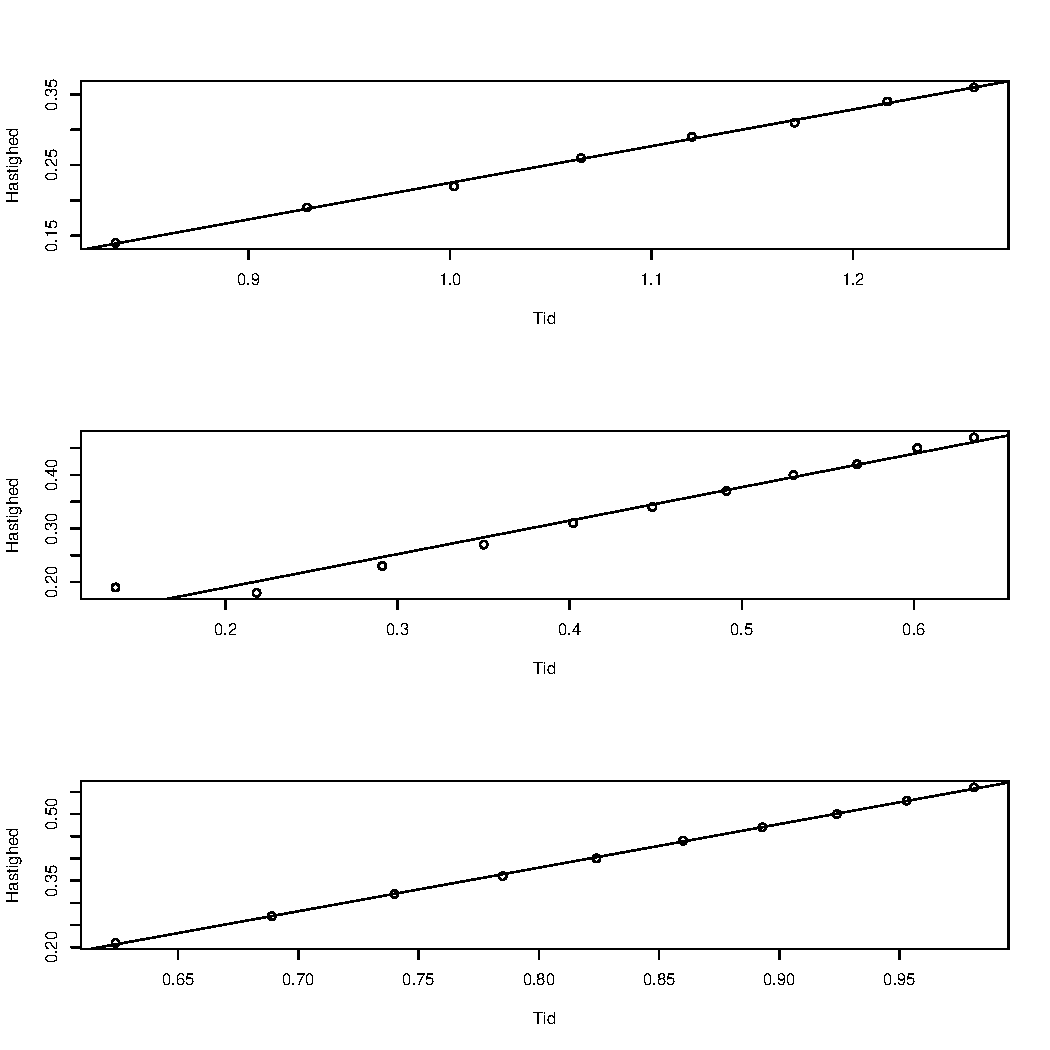
\includegraphics{opgave2.pdf}\\
  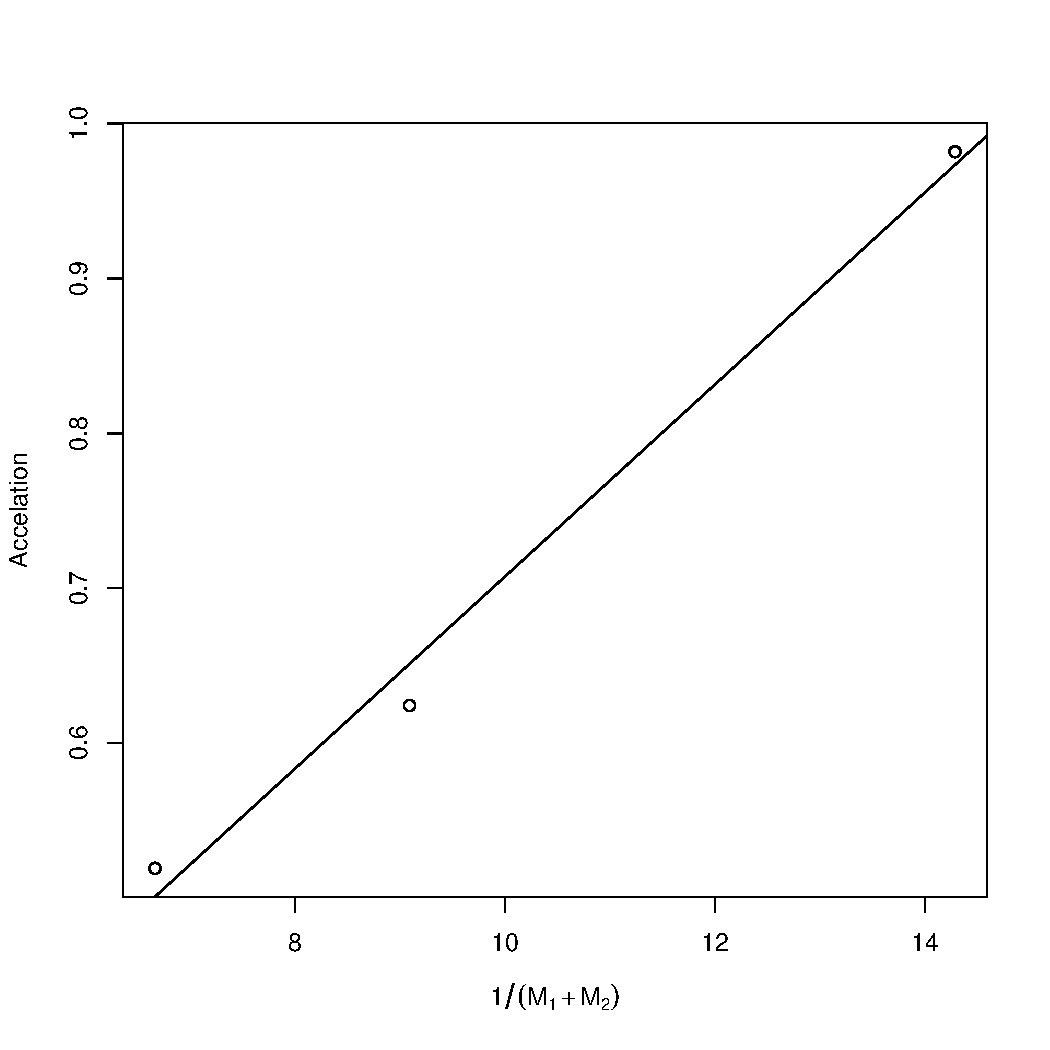
\includegraphics{opgave2acc.pdf}\\
  Så tegner vi \((\frac{1}{M_1+M_2}, a)\) grafen og finder hældningen.
  Hældningen har vi fundet til at være 0.62.\\
  For at kunne sammenligne den med \(F_{res}\) skal vi først udregne
  \(F_{res}\) for de tre måleserier. Til at udregne krafterne bruger vi
  formlen\\
  \[F_{res}=(M_1+M_2) \cdot a\] Så vi udregner de tre krafter til at
  være\\
  \[F_{1}=0.150 \ kg \cdot 0.52 \ \frac{m}{s^2}=0.078 \ N\]
  \[F_{2}=0.110 \ kg \cdot 0.62 \ \frac{m}{s^2}=0.069 \ N\]
  \[F_{3}=0.070 \ kg \cdot 0.98 \ \frac{m}{s^2}=0.069 \ N\] Så hvis vi
  sammenligner de tre med hældningen af grafen som var 0.62. Ser vi at
  de er relativt tætte på hinanden.
\item
  Konkluder på gyldigheden af Newtons 2. lov.f\\
  Hvis vi kigger på vores sammenligning af krafterne fra del 2. ser vi
  at de er meget tæt på hinanden. Og derfor hvis vi kigger bort fra
  fejlkilder kan vi konkludere at newtons 2. lov passer meget godt til
  virkeligheden.
\item
  Undersøg om den mekaniske energi er bevaret under bevægelsen.
  Kommenter resultatet.\\
  Da mekanisk energi er potentiel energi og kinetisk energi lagt sammen,
  finder vi den mekanske energi for de to lodder ved først at finde
  potentiel og kinetisk energi med formlerne\\
  \[E_{potentiel}=m \cdot g \cdot h\] \[E_{kinetisk} = m \cdot v^2\] Det
  gør vi så med alle vores sted og hastigheds værdier og derefter lægger
  dem sammen for at finde den mekaniske energi til alle punkter. Hvis
  den mekaniske energi skulle bevares ville differensen mellem disse
  mekaniske energier være 0. Så vi trækker dem fra hinanden.

  \begin{longtable}[]{@{}r@{}}
  \toprule
  x\tabularnewline
  \midrule
  \endhead
  0.003270\tabularnewline
  0.005439\tabularnewline
  0.006621\tabularnewline
  0.008817\tabularnewline
  0.009994\tabularnewline
  0.012171\tabularnewline
  0.013384\tabularnewline
  0.015512\tabularnewline
  0.016755\tabularnewline
  0.017921\tabularnewline
  0.020077\tabularnewline
  0.022241\tabularnewline
  0.023431\tabularnewline
  0.024520\tabularnewline
  0.026704\tabularnewline
  0.028896\tabularnewline
  0.030114\tabularnewline
  0.032199\tabularnewline
  0.033429\tabularnewline
  0.035649\tabularnewline
  0.036762\tabularnewline
  0.038994\tabularnewline
  0.040113\tabularnewline
  0.041375\tabularnewline
  0.043482\tabularnewline
  0.044609\tabularnewline
  0.046869\tabularnewline
  \bottomrule
  \end{longtable}

  Som vi kan se så er de ikke nul, men de stiger faktisk en lille smule
  for hver gang. Problemet er at vores værdier for hastigheden ikke er
  målt, men de er udregnet af capstone, og derfor er punkter ikke til
  samme tid som stedet.
\end{enumerate}

\section{Fejlkilder}
Vi bruger vores hænder til at give slip for lodderne, så i form af vi bruger vores krop til at i gang sætte faldet kan der være en chance for, at vi påvirker faldet med en
acceleration. Dernæst så beregner Capstone vores acceleration i stedet for at have en mulighed for at måle den, hvilket også skaber en usikkerhed.

